\documentclass[tikz,border=2mm]{standalone}
\begin{document}
	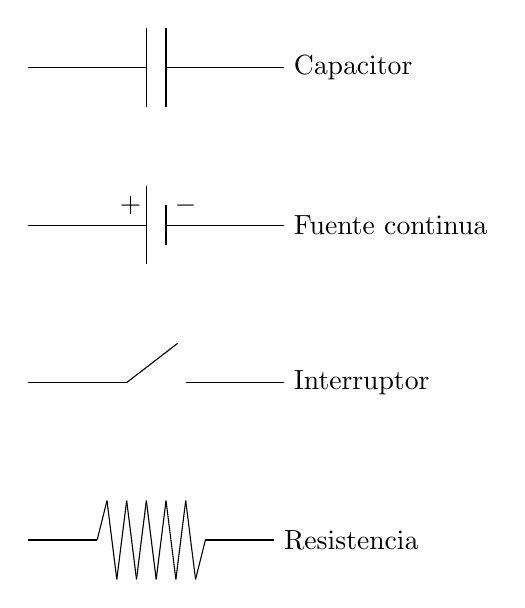
\begin{tikzpicture}
		\draw (0,0) -- (1.5,0);
		\draw (1.5,0.5) -- (1.5,-0.5);
		\draw (1.75,0.5) -- (1.75,-0.5);
		\draw (1.75,0) -- (3.25,0) node[right]{Capacitor};
		
		\draw (0,-2) -- (1.5,-2);
		\draw (1.5,-1.5) -- (1.5,-2.5);
		\node at (1.3,-1.75) {$+$};
		\node at (2,-1.75) {$-$};
		\draw (1.75,-1.75) -- (1.75,-2.25);
		\draw (1.75,-2) -- (3.25,-2) node[right]{Fuente continua};
		
		\draw (0,-4) -- (1.25,-4);
		\draw (1.25,-4) -- (1.9,-3.5);
		\draw (2,-4) -- (3.25,-4) node[right]{Interruptor};
		
		\draw (0,-6) -- (0.875,-6);
		
		\draw (0.875,-6) -- (1,-5.5);
		\draw (1,-5.5) -- (1.125,-6.5);
		\draw (1.125,-6.5) -- (1.25,-5.5);
		\draw (1.25,-5.5) -- (1.375,-6.5);
		\draw (1.375,-6.5) -- (1.5,-5.5);
		\draw (1.5,-5.5) -- (1.625,-6.5);
		\draw (1.625,-6.5) -- (1.75,-5.5);
		\draw (1.75,-5.5) -- (1.875,-6.5);
		\draw (1.875,-6.5) -- (2,-5.5);
		\draw (2,-5.5) -- (2.125,-6.5);
		\draw (2.125,-6.5) -- (2.25,-6);
		
		\draw (2.25,-6) -- (3.125,-6) node[right]{Resistencia};
	\end{tikzpicture}
\end{document}